\documentclass[twoside]{book}

% Packages required by doxygen
\usepackage{fixltx2e}
\usepackage{calc}
\usepackage{doxygen}
\usepackage[export]{adjustbox} % also loads graphicx
\usepackage{graphicx}
\usepackage[utf8]{inputenc}
\usepackage{makeidx}
\usepackage{multicol}
\usepackage{multirow}
\PassOptionsToPackage{warn}{textcomp}
\usepackage{textcomp}
\usepackage[nointegrals]{wasysym}
\usepackage[table]{xcolor}

% NLS support packages
\usepackage[brazil]{babel}
% Font selection
\usepackage[T1]{fontenc}
\usepackage[scaled=.90]{helvet}
\usepackage{courier}
\usepackage{amssymb}
\usepackage{sectsty}
\renewcommand{\familydefault}{\sfdefault}
\allsectionsfont{%
  \fontseries{bc}\selectfont%
  \color{darkgray}%
}
\renewcommand{\DoxyLabelFont}{%
  \fontseries{bc}\selectfont%
  \color{darkgray}%
}
\newcommand{\+}{\discretionary{\mbox{\scriptsize$\hookleftarrow$}}{}{}}

% Page & text layout
\usepackage{geometry}
\geometry{%
  a4paper,%
  top=2.5cm,%
  bottom=2.5cm,%
  left=2.5cm,%
  right=2.5cm%
}
\tolerance=750
\hfuzz=15pt
\hbadness=750
\setlength{\emergencystretch}{15pt}
\setlength{\parindent}{0cm}
\setlength{\parskip}{3ex plus 2ex minus 2ex}
\makeatletter
\renewcommand{\paragraph}{%
  \@startsection{paragraph}{4}{0ex}{-1.0ex}{1.0ex}{%
    \normalfont\normalsize\bfseries\SS@parafont%
  }%
}
\renewcommand{\subparagraph}{%
  \@startsection{subparagraph}{5}{0ex}{-1.0ex}{1.0ex}{%
    \normalfont\normalsize\bfseries\SS@subparafont%
  }%
}
\makeatother

% Headers & footers
\usepackage{fancyhdr}
\pagestyle{fancyplain}
\fancyhead[LE]{\fancyplain{}{\bfseries\thepage}}
\fancyhead[CE]{\fancyplain{}{}}
\fancyhead[RE]{\fancyplain{}{\bfseries\leftmark}}
\fancyhead[LO]{\fancyplain{}{\bfseries\rightmark}}
\fancyhead[CO]{\fancyplain{}{}}
\fancyhead[RO]{\fancyplain{}{\bfseries\thepage}}
\fancyfoot[LE]{\fancyplain{}{}}
\fancyfoot[CE]{\fancyplain{}{}}
\fancyfoot[RE]{\fancyplain{}{\bfseries\scriptsize Gerado por Doxygen }}
\fancyfoot[LO]{\fancyplain{}{\bfseries\scriptsize Gerado por Doxygen }}
\fancyfoot[CO]{\fancyplain{}{}}
\fancyfoot[RO]{\fancyplain{}{}}
\renewcommand{\footrulewidth}{0.4pt}
\renewcommand{\chaptermark}[1]{%
  \markboth{#1}{}%
}
\renewcommand{\sectionmark}[1]{%
  \markright{\thesection\ #1}%
}

% Indices & bibliography
\usepackage{natbib}
\usepackage[titles]{tocloft}
\setcounter{tocdepth}{3}
\setcounter{secnumdepth}{5}
\makeindex

% Hyperlinks (required, but should be loaded last)
\usepackage{ifpdf}
\ifpdf
  \usepackage[pdftex,pagebackref=true]{hyperref}
\else
  \usepackage[ps2pdf,pagebackref=true]{hyperref}
\fi
\hypersetup{%
  colorlinks=true,%
  linkcolor=blue,%
  citecolor=blue,%
  unicode%
}

% Custom commands
\newcommand{\clearemptydoublepage}{%
  \newpage{\pagestyle{empty}\cleardoublepage}%
}

\usepackage{caption}
\captionsetup{labelsep=space,justification=centering,font={bf},singlelinecheck=off,skip=4pt,position=top}

%===== C O N T E N T S =====

\begin{document}

% Titlepage & ToC
\hypersetup{pageanchor=false,
             bookmarksnumbered=true,
             pdfencoding=unicode
            }
\pagenumbering{alph}
\begin{titlepage}
\vspace*{7cm}
\begin{center}%
{\Large Projeto\+P1\+\_\+\+J\+A\+VA }\\
\vspace*{1cm}
{\large Gerado por Doxygen 1.8.14}\\
\end{center}
\end{titlepage}
\clearemptydoublepage
\pagenumbering{roman}
\tableofcontents
\clearemptydoublepage
\pagenumbering{arabic}
\hypersetup{pageanchor=true}

%--- Begin generated contents ---
\chapter{Índice Hierárquico}
\section{Hierarquia de Classes}
Esta lista de hierarquias está parcialmente ordenada (ordem alfabética)\+:\begin{DoxyCompactList}
\item \contentsline{section}{Main}{\pageref{class_main}}{}
\item \contentsline{section}{Mundo}{\pageref{class_mundo}}{}
\item \contentsline{section}{Veiculo}{\pageref{class_veiculo}}{}
\begin{DoxyCompactList}
\item \contentsline{section}{Caminhao}{\pageref{class_caminhao}}{}
\item \contentsline{section}{Carro}{\pageref{class_carro}}{}
\item \contentsline{section}{Moto}{\pageref{class_moto}}{}
\end{DoxyCompactList}
\end{DoxyCompactList}

\chapter{Índice dos Componentes}
\section{Lista de Classes}
Aqui estão as classes, estruturas, uniões e interfaces e suas respectivas descrições\+:\begin{DoxyCompactList}
\item\contentsline{section}{\mbox{\hyperlink{class_caminhao}{Caminhao}} }{\pageref{class_caminhao}}{}
\item\contentsline{section}{\mbox{\hyperlink{class_carro}{Carro}} }{\pageref{class_carro}}{}
\item\contentsline{section}{\mbox{\hyperlink{class_main}{Main}} }{\pageref{class_main}}{}
\item\contentsline{section}{\mbox{\hyperlink{class_moto}{Moto}} }{\pageref{class_moto}}{}
\item\contentsline{section}{\mbox{\hyperlink{class_mundo}{Mundo}} }{\pageref{class_mundo}}{}
\item\contentsline{section}{\mbox{\hyperlink{class_veiculo}{Veiculo}} }{\pageref{class_veiculo}}{}
\end{DoxyCompactList}

\chapter{Classes}
\hypertarget{class_caminhao}{}\section{Referência da Classe Caminhao}
\label{class_caminhao}\index{Caminhao@{Caminhao}}
Diagrama de hierarquia para Caminhao\+:\begin{figure}[H]
\begin{center}
\leavevmode
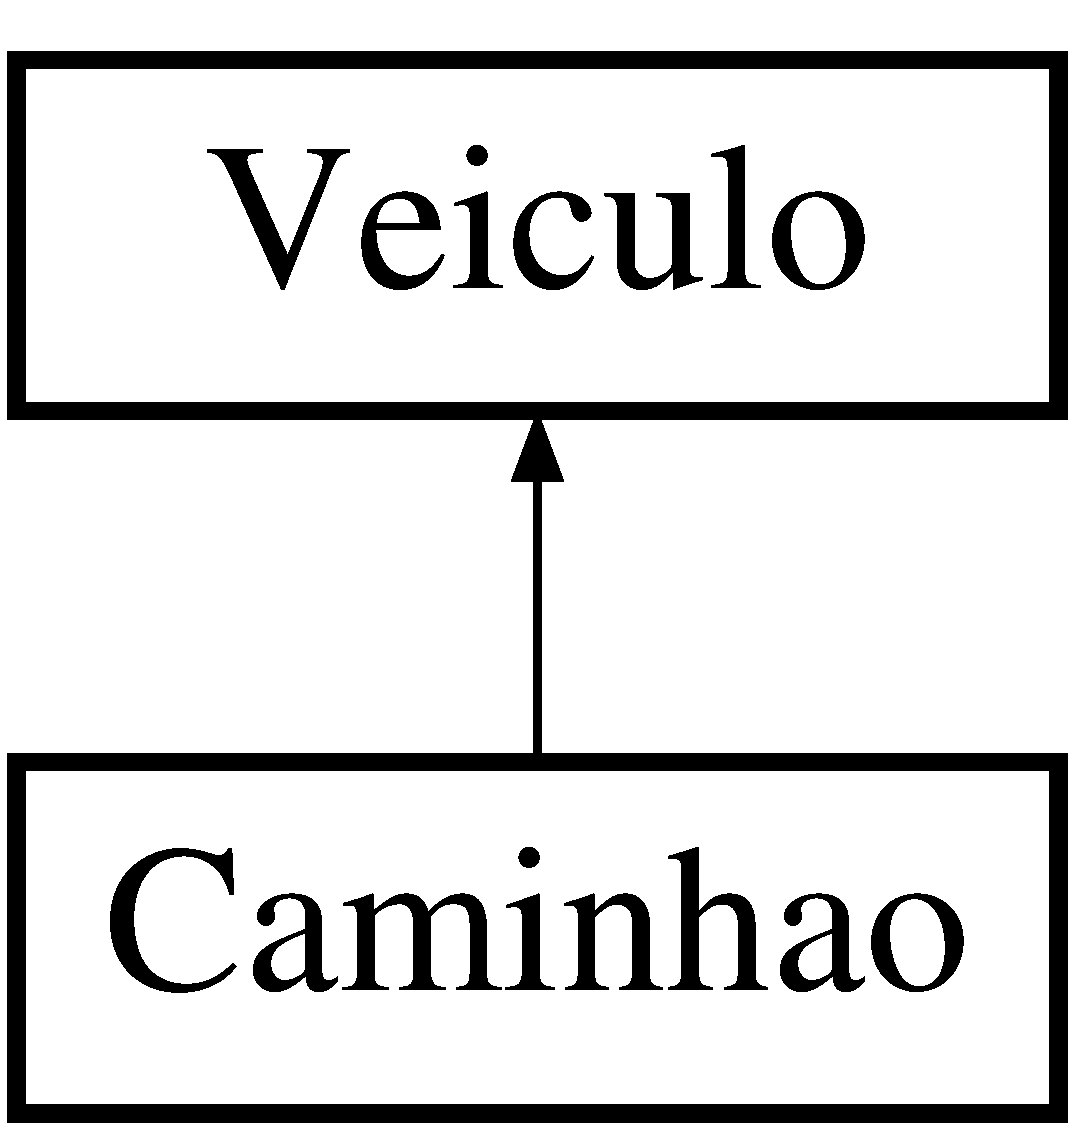
\includegraphics[height=2.000000cm]{class_caminhao}
\end{center}
\end{figure}
\subsection*{Membros Públicos}
\begin{DoxyCompactItemize}
\item 
\mbox{\hyperlink{class_caminhao_af533c39b3db0b14e7c404d4d91a88e47}{Caminhao}} ()
\item 
int \mbox{\hyperlink{class_caminhao_a72a337da0709d0d44385f9a3adc94848}{get\+Carga}} ()
\end{DoxyCompactItemize}
\subsection*{Membros Privados}
\begin{DoxyCompactItemize}
\item 
void \mbox{\hyperlink{class_caminhao_ab8cceb70d87e28684af27ee303804001}{set\+Carga}} ()
\end{DoxyCompactItemize}
\subsection*{Atributos Privados}
\begin{DoxyCompactItemize}
\item 
\mbox{\Hypertarget{class_caminhao_a145576b7d09b5bc02ed6d1328b95e6b9}\label{class_caminhao_a145576b7d09b5bc02ed6d1328b95e6b9}} 
int \mbox{\hyperlink{class_caminhao_a145576b7d09b5bc02ed6d1328b95e6b9}{carga}}
\begin{DoxyCompactList}\small\item\em De 1 a 14 toneladas de carga em um \mbox{\hyperlink{class_caminhao}{Caminhao}}. \end{DoxyCompactList}\end{DoxyCompactItemize}
\subsection*{Outros membros herdados}


\subsection{Descrição detalhada}
Classe \mbox{\hyperlink{class_caminhao}{Caminhao}} que herda da classe \mbox{\hyperlink{class_veiculo}{Veiculo}}. Tem como função criar um objeto \mbox{\hyperlink{class_caminhao}{Caminhao}} e guardar suas especificações. 

\subsection{Construtores e Destrutores}
\mbox{\Hypertarget{class_caminhao_af533c39b3db0b14e7c404d4d91a88e47}\label{class_caminhao_af533c39b3db0b14e7c404d4d91a88e47}} 
\index{Caminhao@{Caminhao}!Caminhao@{Caminhao}}
\index{Caminhao@{Caminhao}!Caminhao@{Caminhao}}
\subsubsection{\texorpdfstring{Caminhao()}{Caminhao()}}
{\footnotesize\ttfamily Caminhao.\+Caminhao (\begin{DoxyParamCaption}{ }\end{DoxyParamCaption})\hspace{0.3cm}{\ttfamily [inline]}}

Construtor padrão. Chama a classe Mãe e chama o set de carga. Chama a classe Mãe entrando a velocidade e cor especificas da classe \mbox{\hyperlink{class_carro}{Carro}}.

Chama o set de carga. 

\subsection{Funções membros}
\mbox{\Hypertarget{class_caminhao_a72a337da0709d0d44385f9a3adc94848}\label{class_caminhao_a72a337da0709d0d44385f9a3adc94848}} 
\index{Caminhao@{Caminhao}!get\+Carga@{get\+Carga}}
\index{get\+Carga@{get\+Carga}!Caminhao@{Caminhao}}
\subsubsection{\texorpdfstring{get\+Carga()}{getCarga()}}
{\footnotesize\ttfamily int Caminhao.\+get\+Carga (\begin{DoxyParamCaption}{ }\end{DoxyParamCaption})\hspace{0.3cm}{\ttfamily [inline]}}

Metodo get para carga. Retorna a carga presente no \mbox{\hyperlink{class_caminhao}{Caminhao}}. \mbox{\Hypertarget{class_caminhao_ab8cceb70d87e28684af27ee303804001}\label{class_caminhao_ab8cceb70d87e28684af27ee303804001}} 
\index{Caminhao@{Caminhao}!set\+Carga@{set\+Carga}}
\index{set\+Carga@{set\+Carga}!Caminhao@{Caminhao}}
\subsubsection{\texorpdfstring{set\+Carga()}{setCarga()}}
{\footnotesize\ttfamily void Caminhao.\+set\+Carga (\begin{DoxyParamCaption}{ }\end{DoxyParamCaption})\hspace{0.3cm}{\ttfamily [inline]}, {\ttfamily [private]}}

Metodo set para carga. Gera uma carga aleatoria entre 1 e 14 toneladas. 

A documentação para essa classe foi gerada a partir do seguinte arquivo\+:\begin{DoxyCompactItemize}
\item 
C\+:/\+Users/\+User/\+Documents/\+Git\+Hub/\+Projeto\+P1\+\_\+\+J\+A\+V\+A/src/Caminhao.\+java\end{DoxyCompactItemize}

\hypertarget{class_carro}{}\section{Referência da Classe Carro}
\label{class_carro}\index{Carro@{Carro}}
Diagrama de hierarquia para Carro\+:\begin{figure}[H]
\begin{center}
\leavevmode
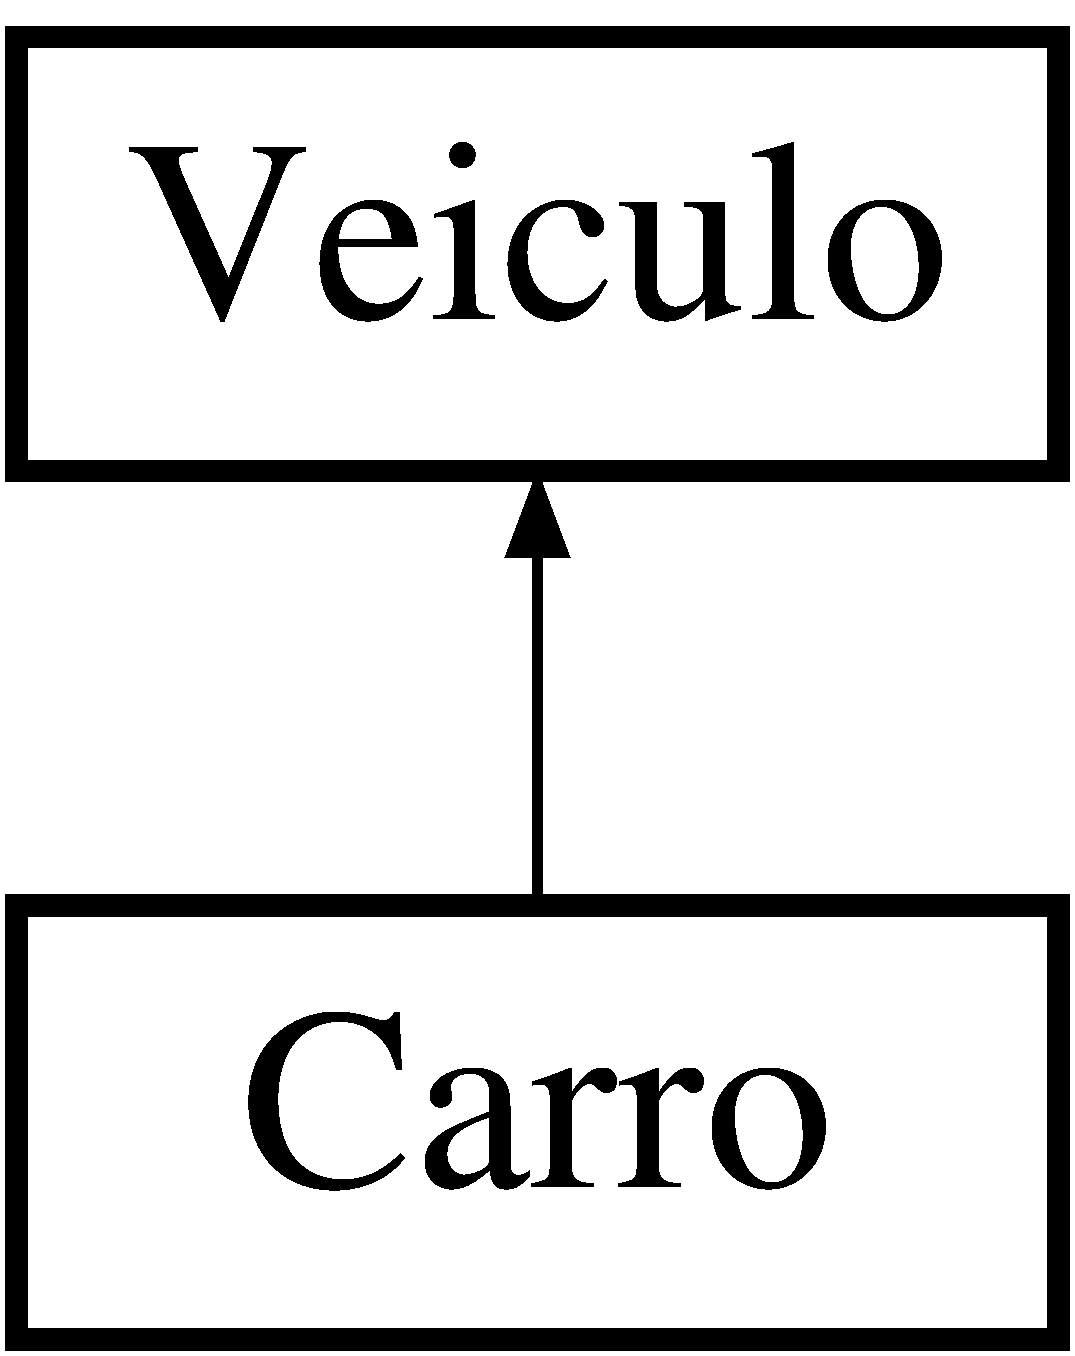
\includegraphics[height=2.000000cm]{class_carro}
\end{center}
\end{figure}
\subsection*{Membros Públicos}
\begin{DoxyCompactItemize}
\item 
\mbox{\hyperlink{class_carro_a853f79365b5c36491d34cf8f3815f75e}{Carro}} ()
\item 
int \mbox{\hyperlink{class_carro_a5c4e195d2148e78186532d315630a7a1}{get\+Passageiros}} ()
\end{DoxyCompactItemize}
\subsection*{Membros Privados}
\begin{DoxyCompactItemize}
\item 
void \mbox{\hyperlink{class_carro_a154dc6a973a0b8e345bffcdfd4721615}{set\+Passageiros}} ()
\end{DoxyCompactItemize}
\subsection*{Atributos Privados}
\begin{DoxyCompactItemize}
\item 
\mbox{\Hypertarget{class_carro_af752fd9ef168621245eb8c3d4eee45e1}\label{class_carro_af752fd9ef168621245eb8c3d4eee45e1}} 
int \mbox{\hyperlink{class_carro_af752fd9ef168621245eb8c3d4eee45e1}{passageiros}}
\begin{DoxyCompactList}\small\item\em De 1 a 4 passageiros em um \mbox{\hyperlink{class_carro}{Carro}}. \end{DoxyCompactList}\end{DoxyCompactItemize}
\subsection*{Outros membros herdados}


\subsection{Descrição detalhada}
Classe \mbox{\hyperlink{class_carro}{Carro}} que herda da classe \mbox{\hyperlink{class_veiculo}{Veiculo}}. Tem como função criar um objeto \mbox{\hyperlink{class_carro}{Carro}} e guardar suas especificações. 

\subsection{Construtores e Destrutores}
\mbox{\Hypertarget{class_carro_a853f79365b5c36491d34cf8f3815f75e}\label{class_carro_a853f79365b5c36491d34cf8f3815f75e}} 
\index{Carro@{Carro}!Carro@{Carro}}
\index{Carro@{Carro}!Carro@{Carro}}
\subsubsection{\texorpdfstring{Carro()}{Carro()}}
{\footnotesize\ttfamily Carro.\+Carro (\begin{DoxyParamCaption}{ }\end{DoxyParamCaption})\hspace{0.3cm}{\ttfamily [inline]}}

Construtor padrão. Chama a classe Mãe e chama o set de passageiros. Chama a classe Mãe entrando a velocidade e cor especificas da classe \mbox{\hyperlink{class_carro}{Carro}}.

Chama o set de passageiros. 

\subsection{Funções membros}
\mbox{\Hypertarget{class_carro_a5c4e195d2148e78186532d315630a7a1}\label{class_carro_a5c4e195d2148e78186532d315630a7a1}} 
\index{Carro@{Carro}!get\+Passageiros@{get\+Passageiros}}
\index{get\+Passageiros@{get\+Passageiros}!Carro@{Carro}}
\subsubsection{\texorpdfstring{get\+Passageiros()}{getPassageiros()}}
{\footnotesize\ttfamily int Carro.\+get\+Passageiros (\begin{DoxyParamCaption}{ }\end{DoxyParamCaption})\hspace{0.3cm}{\ttfamily [inline]}}

Metodo get de passageiros. retorna o numero de passageiros no \mbox{\hyperlink{class_carro}{Carro}}. \mbox{\Hypertarget{class_carro_a154dc6a973a0b8e345bffcdfd4721615}\label{class_carro_a154dc6a973a0b8e345bffcdfd4721615}} 
\index{Carro@{Carro}!set\+Passageiros@{set\+Passageiros}}
\index{set\+Passageiros@{set\+Passageiros}!Carro@{Carro}}
\subsubsection{\texorpdfstring{set\+Passageiros()}{setPassageiros()}}
{\footnotesize\ttfamily void Carro.\+set\+Passageiros (\begin{DoxyParamCaption}{ }\end{DoxyParamCaption})\hspace{0.3cm}{\ttfamily [inline]}, {\ttfamily [private]}}

Metodo set para passageiros. Gera um numero aleatorio de passageiros entre 1 e 4. 

A documentação para essa classe foi gerada a partir do seguinte arquivo\+:\begin{DoxyCompactItemize}
\item 
C\+:/\+Users/\+User/\+Documents/\+Git\+Hub/\+Projeto\+P1\+\_\+\+J\+A\+V\+A/src/Carro.\+java\end{DoxyCompactItemize}

\hypertarget{class_main}{}\section{Referência da Classe Main}
\label{class_main}\index{Main@{Main}}
\subsection*{Membros Públicos Estáticos}
\begin{DoxyCompactItemize}
\item 
static void \mbox{\hyperlink{class_main_a8a5d0f827edddff706cc0e6740d0579a}{main}} (String\mbox{[}$\,$\mbox{]} args)
\end{DoxyCompactItemize}


\subsection{Descrição detalhada}
Classe executavel do programa. É ela que contem todas as chamadas de função para o funcionamento do mesmo. 

\subsection{Funções membros}
\mbox{\Hypertarget{class_main_a8a5d0f827edddff706cc0e6740d0579a}\label{class_main_a8a5d0f827edddff706cc0e6740d0579a}} 
\index{Main@{Main}!main@{main}}
\index{main@{main}!Main@{Main}}
\subsubsection{\texorpdfstring{main()}{main()}}
{\footnotesize\ttfamily static void Main.\+main (\begin{DoxyParamCaption}\item[{String \mbox{[}$\,$\mbox{]}}]{args }\end{DoxyParamCaption})\hspace{0.3cm}{\ttfamily [inline]}, {\ttfamily [static]}}

Cria um \mbox{\hyperlink{class_mundo}{Mundo}}.

Cria uma lista de caminhões da classe \mbox{\hyperlink{class_caminhao}{Caminhao}}.

Cria uma lista de carros da classe \mbox{\hyperlink{class_carro}{Carro}}.

Cria uma lista de motos da classe \mbox{\hyperlink{class_moto}{Moto}}.

For que adiciona 10 novos veiculos de cada tipo para o teste do mundo de grades.

$<$ contador para limitar o numero de prints.

While que permite o programa rodar até o momento em que apenas um tipo de veiculo sobrar ou os prints excederem o limite que impus.

Volta o mapa a sua forma original.

For que percorre cada caminhao.

Move o caminhão.

For que percorre cada carro.

Move o carro.

For que percorre cada moto.

Move a moto.

Atualiza o mundo.

Conta cada print no objetivo de evitar o excesso de prints, para que não seja uma run \char`\"{}infinita\char`\"{}.

Manda um aviso de que ja foram atingidos 10000 prints.

Pausa o programa durante um tempo determinado em milisegundos.

A documentação para essa classe foi gerada a partir do seguinte arquivo\+:\begin{DoxyCompactItemize}
\item 
C\+:/\+Users/\+User/\+Documents/\+Git\+Hub/\+Projeto\+P1\+\_\+\+J\+A\+V\+A/src/Main.\+java\end{DoxyCompactItemize}

\hypertarget{class_moto}{}\section{Referência da Classe Moto}
\label{class_moto}\index{Moto@{Moto}}
Diagrama de hierarquia para Moto\+:\begin{figure}[H]
\begin{center}
\leavevmode
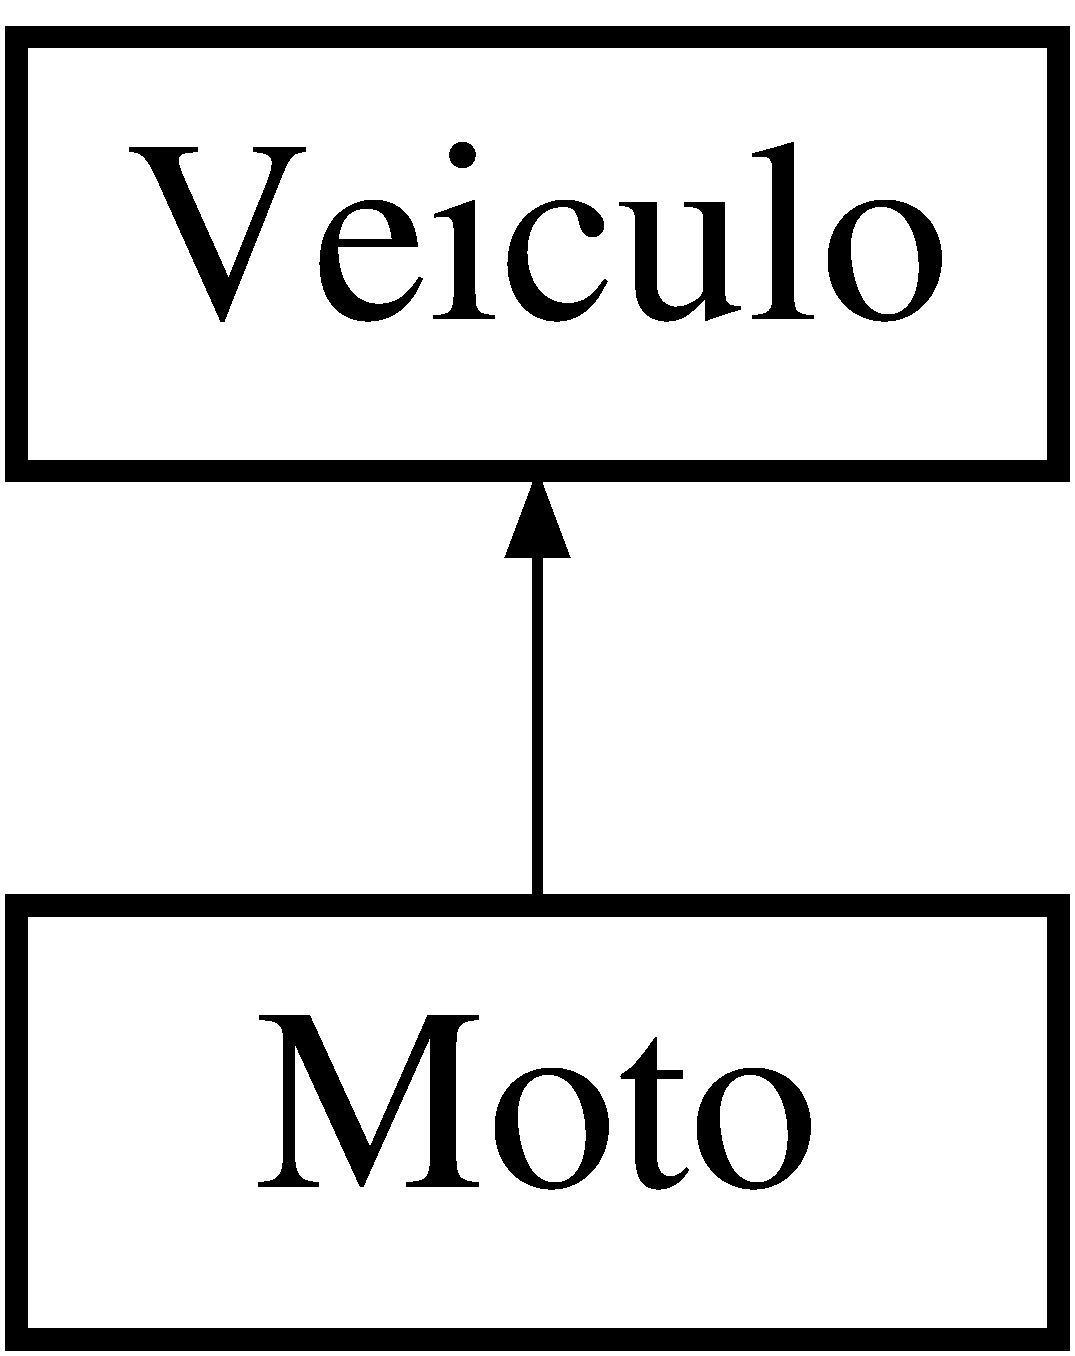
\includegraphics[height=2.000000cm]{class_moto}
\end{center}
\end{figure}
\subsection*{Membros Públicos}
\begin{DoxyCompactItemize}
\item 
\mbox{\hyperlink{class_moto_af900d6c1d6b9a69fb6b8bdb0c3401603}{Moto}} ()
\item 
int \mbox{\hyperlink{class_moto_af285d528cc9d6e1dd47db8d7a36a08bd}{get\+Passageiros}} ()
\end{DoxyCompactItemize}
\subsection*{Membros Privados}
\begin{DoxyCompactItemize}
\item 
void \mbox{\hyperlink{class_moto_a336f2ac21dee386aef726c3207b113f9}{set\+Passageiros}} ()
\end{DoxyCompactItemize}
\subsection*{Atributos Privados}
\begin{DoxyCompactItemize}
\item 
\mbox{\Hypertarget{class_moto_a5cf8ea81e47701cfc6a132fdc046071d}\label{class_moto_a5cf8ea81e47701cfc6a132fdc046071d}} 
int \mbox{\hyperlink{class_moto_a5cf8ea81e47701cfc6a132fdc046071d}{passageiros}}
\begin{DoxyCompactList}\small\item\em De 1 a 2 passageiros em uma \mbox{\hyperlink{class_moto}{Moto}}. \end{DoxyCompactList}\end{DoxyCompactItemize}
\subsection*{Outros membros herdados}


\subsection{Descrição detalhada}
Classe \mbox{\hyperlink{class_moto}{Moto}} que herda da classe \mbox{\hyperlink{class_veiculo}{Veiculo}}. Tem como função criar um objeto \mbox{\hyperlink{class_moto}{Moto}} e guardar suas especificações. 

\subsection{Construtores e Destrutores}
\mbox{\Hypertarget{class_moto_af900d6c1d6b9a69fb6b8bdb0c3401603}\label{class_moto_af900d6c1d6b9a69fb6b8bdb0c3401603}} 
\index{Moto@{Moto}!Moto@{Moto}}
\index{Moto@{Moto}!Moto@{Moto}}
\subsubsection{\texorpdfstring{Moto()}{Moto()}}
{\footnotesize\ttfamily Moto.\+Moto (\begin{DoxyParamCaption}{ }\end{DoxyParamCaption})\hspace{0.3cm}{\ttfamily [inline]}}

Construtor padrão. Chama a classe Mãe e chama o set de passageiros. Chama a classe Mãe entrando a velocidade e cor especificas da classe \mbox{\hyperlink{class_moto}{Moto}}.

Chama o set de passageiros. 

\subsection{Funções membros}
\mbox{\Hypertarget{class_moto_af285d528cc9d6e1dd47db8d7a36a08bd}\label{class_moto_af285d528cc9d6e1dd47db8d7a36a08bd}} 
\index{Moto@{Moto}!get\+Passageiros@{get\+Passageiros}}
\index{get\+Passageiros@{get\+Passageiros}!Moto@{Moto}}
\subsubsection{\texorpdfstring{get\+Passageiros()}{getPassageiros()}}
{\footnotesize\ttfamily int Moto.\+get\+Passageiros (\begin{DoxyParamCaption}{ }\end{DoxyParamCaption})\hspace{0.3cm}{\ttfamily [inline]}}

Metodo get de passageiros. retorna o numero de passageiros na \mbox{\hyperlink{class_moto}{Moto}}. \mbox{\Hypertarget{class_moto_a336f2ac21dee386aef726c3207b113f9}\label{class_moto_a336f2ac21dee386aef726c3207b113f9}} 
\index{Moto@{Moto}!set\+Passageiros@{set\+Passageiros}}
\index{set\+Passageiros@{set\+Passageiros}!Moto@{Moto}}
\subsubsection{\texorpdfstring{set\+Passageiros()}{setPassageiros()}}
{\footnotesize\ttfamily void Moto.\+set\+Passageiros (\begin{DoxyParamCaption}{ }\end{DoxyParamCaption})\hspace{0.3cm}{\ttfamily [inline]}, {\ttfamily [private]}}

Metodo set para passageiros. Gera um numero aleatorio de passageiros entre 1 e 2. 

A documentação para essa classe foi gerada a partir do seguinte arquivo\+:\begin{DoxyCompactItemize}
\item 
C\+:/\+Users/\+User/\+Documents/\+Git\+Hub/\+Projeto\+P1\+\_\+\+J\+A\+V\+A/src/Moto.\+java\end{DoxyCompactItemize}

\hypertarget{class_mundo}{}\section{Referência da Classe Mundo}
\label{class_mundo}\index{Mundo@{Mundo}}
\subsection*{Membros Públicos}
\begin{DoxyCompactItemize}
\item 
\mbox{\hyperlink{class_mundo_ae3801a0a633ad3475456c67639561105}{Mundo}} ()
\item 
void \mbox{\hyperlink{class_mundo_af5231bba26317e2ff2eb04e9bf0ac495}{att\+Mapa}} ()
\item 
void \mbox{\hyperlink{class_mundo_a6992f445c8947937e73492a0ac6895fa}{att\+Mundo}} (Array\+List$<$ \mbox{\hyperlink{class_caminhao}{Caminhao}} $>$ caminhoes, Array\+List$<$ \mbox{\hyperlink{class_carro}{Carro}} $>$ carros, Array\+List$<$ \mbox{\hyperlink{class_moto}{Moto}} $>$ motos)
\item 
void \mbox{\hyperlink{class_mundo_abe2d4fb96005c19b423cc6163bf986f5}{print\+Mundo}} ()
\end{DoxyCompactItemize}
\subsection*{Atributos Privados}
\begin{DoxyCompactItemize}
\item 
int \mbox{\hyperlink{class_mundo_a8332b2d52b9f317338a4d6cbe10bbcbb}{mapa}} \mbox{[}$\,$\mbox{]}\mbox{[}$\,$\mbox{]}
\item 
\mbox{\Hypertarget{class_mundo_afccad9fd3eda103dc801ffaf2c391e1a}\label{class_mundo_afccad9fd3eda103dc801ffaf2c391e1a}} 
int \mbox{\hyperlink{class_mundo_afccad9fd3eda103dc801ffaf2c391e1a}{attmapa}} \mbox{[}$\,$\mbox{]}\mbox{[}$\,$\mbox{]}
\begin{DoxyCompactList}\small\item\em \mbox{\hyperlink{class_mundo}{Mundo}} de grades para atualizações de posição. \end{DoxyCompactList}\item 
\mbox{\Hypertarget{class_mundo_afa552f3d464f7372e35f182ad60f0e2c}\label{class_mundo_afa552f3d464f7372e35f182ad60f0e2c}} 
int \mbox{\hyperlink{class_mundo_afa552f3d464f7372e35f182ad60f0e2c}{cont\+Vitimas}}
\begin{DoxyCompactList}\small\item\em Contador de vitimas em batidas. \end{DoxyCompactList}\item 
\mbox{\Hypertarget{class_mundo_a6289b5c83662e0f64c6d673983581dc3}\label{class_mundo_a6289b5c83662e0f64c6d673983581dc3}} 
int \mbox{\hyperlink{class_mundo_a6289b5c83662e0f64c6d673983581dc3}{cont\+Carga}}
\begin{DoxyCompactList}\small\item\em Contador de carga perdida em batidas. \end{DoxyCompactList}\end{DoxyCompactItemize}


\subsection{Descrição detalhada}
Classe para criação de um \mbox{\hyperlink{class_mundo}{Mundo}} de grades. Capaz de montar um mundo de grades de forma colorida e decidir como o \mbox{\hyperlink{class_mundo}{Mundo}} vai reagir em relação as classes \mbox{\hyperlink{class_veiculo}{Veiculo}}. 

\subsection{Construtores e Destrutores}
\mbox{\Hypertarget{class_mundo_ae3801a0a633ad3475456c67639561105}\label{class_mundo_ae3801a0a633ad3475456c67639561105}} 
\index{Mundo@{Mundo}!Mundo@{Mundo}}
\index{Mundo@{Mundo}!Mundo@{Mundo}}
\subsubsection{\texorpdfstring{Mundo()}{Mundo()}}
{\footnotesize\ttfamily Mundo.\+Mundo (\begin{DoxyParamCaption}{ }\end{DoxyParamCaption})\hspace{0.3cm}{\ttfamily [inline]}}

Construtor padrão de \mbox{\hyperlink{class_mundo}{Mundo}}. Cria um mundo para atualizações, com sua forma inicial. $<$ \mbox{\hyperlink{class_mundo}{Mundo}} de grades 40 x 40, 0 = vazio, 1 = bordas, 2 = fabricas. Serve para criar um mundo como o mapa original. 

\subsection{Funções membros}
\mbox{\Hypertarget{class_mundo_af5231bba26317e2ff2eb04e9bf0ac495}\label{class_mundo_af5231bba26317e2ff2eb04e9bf0ac495}} 
\index{Mundo@{Mundo}!att\+Mapa@{att\+Mapa}}
\index{att\+Mapa@{att\+Mapa}!Mundo@{Mundo}}
\subsubsection{\texorpdfstring{att\+Mapa()}{attMapa()}}
{\footnotesize\ttfamily void Mundo.\+att\+Mapa (\begin{DoxyParamCaption}{ }\end{DoxyParamCaption})\hspace{0.3cm}{\ttfamily [inline]}}

Método para atualização do mapa. Atualiza o mapa para sua versão original, para realocação e interação de cada \mbox{\hyperlink{class_veiculo}{Veiculo}}. $<$ \mbox{\hyperlink{class_mundo}{Mundo}} de grades 40 x 40, 0 = vazio, 1 = bordas, 2 = fabricas. Serve para atualizar posições. \mbox{\Hypertarget{class_mundo_a6992f445c8947937e73492a0ac6895fa}\label{class_mundo_a6992f445c8947937e73492a0ac6895fa}} 
\index{Mundo@{Mundo}!att\+Mundo@{att\+Mundo}}
\index{att\+Mundo@{att\+Mundo}!Mundo@{Mundo}}
\subsubsection{\texorpdfstring{att\+Mundo()}{attMundo()}}
{\footnotesize\ttfamily void Mundo.\+att\+Mundo (\begin{DoxyParamCaption}\item[{Array\+List$<$ \mbox{\hyperlink{class_caminhao}{Caminhao}} $>$}]{caminhoes,  }\item[{Array\+List$<$ \mbox{\hyperlink{class_carro}{Carro}} $>$}]{carros,  }\item[{Array\+List$<$ \mbox{\hyperlink{class_moto}{Moto}} $>$}]{motos }\end{DoxyParamCaption})\hspace{0.3cm}{\ttfamily [inline]}}

Método para atualização do \mbox{\hyperlink{class_mundo}{Mundo}}. Percorre cada tipo de \mbox{\hyperlink{class_veiculo}{Veiculo}} para confirmar se\+: ele está em um espaço vazio, em uma borda, em uma fabrica ou em cima de outro \mbox{\hyperlink{class_veiculo}{Veiculo}}; onde a fabrica duplica veiculos, os veiculos que batem dependendo de quem é \textquotesingle{}maior\textquotesingle{}, vai sair ganhando ou se ambos forem iguais ambos \textquotesingle{}morrem\textquotesingle{}. Declarando x e y, que seram usados para saber a posição exata de cada \mbox{\hyperlink{class_veiculo}{Veiculo}} criado.

percorre todo o Arraylist de \mbox{\hyperlink{class_moto}{Moto}}.

Da para x o valor da posição x do \mbox{\hyperlink{class_moto}{Moto}}.

Da para y o valor da posição y do \mbox{\hyperlink{class_moto}{Moto}}.

Se a \mbox{\hyperlink{class_moto}{Moto}} se movimentou para uma borda ou uma área vazia, entra neste if.

Seta fabrica como false. Afinal a \mbox{\hyperlink{class_moto}{Moto}} está fora da fabrica.

Seta a cor do mapa para o valor que está em \mbox{\hyperlink{class_moto}{Moto}}.

Cria nova \mbox{\hyperlink{class_moto}{Moto}}. Se uma \mbox{\hyperlink{class_moto}{Moto}} se depara com uma fabrica ela se duplica.

Só entra no if se a fabrica ainda não foi visitada no movimento anterior.

Seta a fabrica como true. Para que uma \mbox{\hyperlink{class_moto}{Moto}} não repita sua duplicação sem antes sair e voltar a fabrica. ~\newline
~\newline
~\newline
~\newline
~\newline
~\newline
~\newline
~\newline
~\newline
~\newline
~\newline
~\newline
~\newline
~\newline
~\newline
~\newline
~\newline
~\newline
~\newline
~\newline
~\newline
~\newline
~\newline
~\newline
~\newline
~\newline
~\newline
~\newline
~\newline
~\newline
~\newline
~\newline
~\newline
~\newline
~\newline
~\newline
~\newline
~\newline
~\newline
~\newline
~\newline
~\newline
~\newline
~\newline
~\newline
~\newline
~\newline
~\newline
~\newline
~\newline
~\newline
~\newline
~\newline
~\newline
~\newline
~\newline
~\newline
~\newline
~\newline
~\newline
~\newline
~\newline
~\newline
~\newline
~\newline
~\newline
~\newline
~\newline
~\newline
~\newline
~\newline
~\newline
~\newline
~\newline
~\newline
~\newline
~\newline
~\newline
~\newline
~\newline
~\newline
~\newline
~\newline
 Adiciona uma nova \mbox{\hyperlink{class_moto}{Moto}} se o \mbox{\hyperlink{class_veiculo}{Veiculo}} visitou a fabrica.

Seta a cor do mapa para o valor que está em \mbox{\hyperlink{class_moto}{Moto}}.

Exclui as motos batidas. Se uma \mbox{\hyperlink{class_moto}{Moto}} se depara com outra \mbox{\hyperlink{class_moto}{Moto}}, então será nescessario excluir ambas. ~\newline
~\newline
~\newline
~\newline
~\newline
~\newline
~\newline
~\newline
~\newline
~\newline
~\newline
~\newline
~\newline
~\newline
~\newline
~\newline
~\newline
~\newline
~\newline
~\newline
~\newline
~\newline
~\newline
~\newline
~\newline
~\newline
~\newline
~\newline
~\newline
~\newline
~\newline
~\newline
~\newline
~\newline
~\newline
~\newline
~\newline
~\newline
~\newline
~\newline
~\newline
~\newline
~\newline
~\newline
~\newline
~\newline
~\newline
~\newline
~\newline
~\newline
~\newline
~\newline
~\newline
~\newline
~\newline
~\newline
~\newline
~\newline
~\newline
~\newline
~\newline
~\newline
~\newline
~\newline
~\newline
~\newline
~\newline
~\newline
~\newline
~\newline
~\newline
~\newline
~\newline
~\newline
~\newline
~\newline
~\newline
~\newline
~\newline
~\newline
 Percorre todas as motos que ja existem para descobrir quem bateu.

Se for a \mbox{\hyperlink{class_moto}{Moto}} que sofreu a batida entra no if.

Adiciona os passageiros da \mbox{\hyperlink{class_moto}{Moto}} ao contador de vitimas.

Remove o \mbox{\hyperlink{class_moto}{Moto}} que sofreu a batida.

Para sair do for no momento em que achar a \mbox{\hyperlink{class_moto}{Moto}} que sofreu o acidente.

Voltando no array pois uma \mbox{\hyperlink{class_moto}{Moto}} que bateu foi retirado de la, assim precisando voltar atraz para retirar o proximo que sofreu a batida. ~\newline
~\newline
~\newline
~\newline
~\newline
~\newline
~\newline
~\newline
~\newline
~\newline
~\newline
~\newline
~\newline
~\newline
~\newline
~\newline
~\newline
~\newline
~\newline
~\newline
~\newline
~\newline
~\newline
~\newline
~\newline
~\newline
~\newline
~\newline
~\newline
~\newline
~\newline
~\newline
~\newline
~\newline
~\newline
~\newline
~\newline
~\newline
~\newline
~\newline
~\newline
~\newline
~\newline
~\newline
~\newline
~\newline
~\newline
~\newline
~\newline
~\newline
~\newline
~\newline
~\newline
~\newline
~\newline
~\newline
~\newline
~\newline
~\newline
~\newline
~\newline
~\newline
~\newline
~\newline
~\newline
~\newline
~\newline
~\newline
~\newline
~\newline
~\newline
~\newline
~\newline
~\newline
 Adiciona os passageiros da \mbox{\hyperlink{class_moto}{Moto}} ao contador de vitimas.

Remove o \mbox{\hyperlink{class_moto}{Moto}} que sofreu a batida. ~\newline
~\newline
~\newline
~\newline
~\newline
~\newline
~\newline
~\newline
~\newline
~\newline
~\newline
~\newline
~\newline
~\newline
~\newline
~\newline
~\newline
~\newline
~\newline
~\newline
~\newline
~\newline
~\newline
~\newline
~\newline
~\newline
~\newline
~\newline
~\newline
~\newline
~\newline
~\newline
~\newline
~\newline
~\newline
~\newline
~\newline
~\newline
~\newline
~\newline
~\newline
~\newline
~\newline
~\newline
~\newline
~\newline
~\newline
~\newline
~\newline
~\newline
~\newline
~\newline
~\newline
~\newline
~\newline
~\newline
~\newline
~\newline
~\newline
~\newline
~\newline
~\newline
~\newline
~\newline
~\newline
~\newline
~\newline
~\newline
~\newline
~\newline
~\newline
~\newline
 voltando no array pois uma \mbox{\hyperlink{class_moto}{Moto}} que bateu e foi retirado de la, assim precisando voltar atraz para continuar o for vizualizando todos as motos que faltaram. ~\newline
~\newline
~\newline
~\newline
~\newline
~\newline
~\newline
~\newline
~\newline
~\newline
~\newline
~\newline
~\newline
~\newline
~\newline
~\newline
~\newline
~\newline
~\newline
~\newline
~\newline
~\newline
~\newline
~\newline
~\newline
~\newline
~\newline
~\newline
~\newline
~\newline
~\newline
~\newline
~\newline
~\newline
~\newline
~\newline
~\newline
~\newline
~\newline
~\newline
~\newline
~\newline
~\newline
~\newline
~\newline
~\newline
~\newline
~\newline
~\newline
~\newline
~\newline
~\newline
~\newline
~\newline
~\newline
~\newline
~\newline
~\newline
~\newline
~\newline
~\newline
~\newline
~\newline
~\newline
~\newline
~\newline
~\newline
~\newline
~\newline
~\newline
~\newline
 o ponto da batida será substituido pelo valor no mapa original.

percorre todo o Arraylist de \mbox{\hyperlink{class_carro}{Carro}}.

Da para x o valor da posição x do \mbox{\hyperlink{class_carro}{Carro}}.

Da para y o valor da posição y do \mbox{\hyperlink{class_carro}{Carro}}.

Se o \mbox{\hyperlink{class_carro}{Carro}} se movimentou para uma borda ou uma área vazia, entra neste if.

Seta fabrica como false. Afinal o \mbox{\hyperlink{class_carro}{Carro}} está fora da fabrica.

Seta a cor do mapa para o valor que está em \mbox{\hyperlink{class_carro}{Carro}}.

Cria novo \mbox{\hyperlink{class_carro}{Carro}}. Se um \mbox{\hyperlink{class_carro}{Carro}} se depara com uma fabrica ele se duplica.

Só entra no if se a fabrica ainda não foi visitada no movimento anterior.

Seta a fabrica como true. Para que um carro não repita sua duplicação sem antes sair e voltar a fabrica. ~\newline
~\newline
~\newline
~\newline
~\newline
~\newline
~\newline
~\newline
~\newline
~\newline
~\newline
~\newline
~\newline
~\newline
~\newline
~\newline
~\newline
~\newline
~\newline
~\newline
~\newline
~\newline
~\newline
~\newline
~\newline
~\newline
~\newline
~\newline
~\newline
~\newline
~\newline
~\newline
~\newline
~\newline
~\newline
~\newline
~\newline
~\newline
~\newline
~\newline
~\newline
~\newline
~\newline
~\newline
~\newline
~\newline
~\newline
~\newline
~\newline
~\newline
~\newline
~\newline
~\newline
~\newline
~\newline
~\newline
~\newline
~\newline
~\newline
~\newline
~\newline
 Adiciona um novo \mbox{\hyperlink{class_carro}{Carro}} se o \mbox{\hyperlink{class_veiculo}{Veiculo}} visitou a fabrica.

Seta a cor do mapa para o valor que está em \mbox{\hyperlink{class_carro}{Carro}}.

Exclui as motos batidas. Se um \mbox{\hyperlink{class_carro}{Carro}} se depara com uma \mbox{\hyperlink{class_moto}{Moto}}, a \mbox{\hyperlink{class_moto}{Moto}} \char`\"{}morre\char`\"{}.

Percorre todas as motos para descobrir quem bateu.

Se for a \mbox{\hyperlink{class_moto}{Moto}} que sofreu a batida entra no if.

Adiciona os passageiros da \mbox{\hyperlink{class_moto}{Moto}} ao contador de vitimas.

Remove o \mbox{\hyperlink{class_moto}{Moto}} que sofreu a batida.

Para sair do for no momento em que achar o \mbox{\hyperlink{class_moto}{Moto}} que sofreu o acidente.

Seta a cor do mapa para o valor que está em \mbox{\hyperlink{class_carro}{Carro}}.

Exclui os carros batidos. Se um \mbox{\hyperlink{class_carro}{Carro}} se depara com outro \mbox{\hyperlink{class_carro}{Carro}}, então será nescessario excluir ambos. ~\newline
~\newline
~\newline
~\newline
~\newline
~\newline
~\newline
~\newline
~\newline
~\newline
~\newline
~\newline
~\newline
~\newline
~\newline
~\newline
~\newline
~\newline
~\newline
~\newline
~\newline
~\newline
~\newline
~\newline
~\newline
~\newline
~\newline
~\newline
~\newline
~\newline
~\newline
~\newline
~\newline
~\newline
~\newline
~\newline
~\newline
~\newline
~\newline
~\newline
~\newline
~\newline
~\newline
~\newline
~\newline
~\newline
~\newline
~\newline
~\newline
~\newline
~\newline
 Percorre todos os carros que ja existem para descobrir quem bateu.

Se for o \mbox{\hyperlink{class_carro}{Carro}} que sofreu a batida entra no if.

Adiciona os passageiros do \mbox{\hyperlink{class_carro}{Carro}} ao contador de vitimas.

Remove o \mbox{\hyperlink{class_carro}{Carro}} que sofreu a batida.

Para sair do for no momento em que achar o \mbox{\hyperlink{class_carro}{Carro}} que sofreu o acidente.

Voltando no array pois um \mbox{\hyperlink{class_carro}{Carro}} que bateu foi retirado de la, assim precisando voltar atraz para retirar o proximo que sofreu a batida. ~\newline
~\newline
~\newline
~\newline
~\newline
~\newline
~\newline
~\newline
~\newline
~\newline
~\newline
~\newline
~\newline
~\newline
~\newline
~\newline
~\newline
~\newline
~\newline
~\newline
~\newline
~\newline
~\newline
~\newline
~\newline
~\newline
~\newline
~\newline
~\newline
~\newline
~\newline
~\newline
~\newline
~\newline
~\newline
~\newline
~\newline
~\newline
~\newline
~\newline
~\newline
~\newline
~\newline
~\newline
~\newline
 Adiciona os passageiros do \mbox{\hyperlink{class_carro}{Carro}} ao contador de vitimas.

Remove o \mbox{\hyperlink{class_carro}{Carro}} que sofreu a batida. ~\newline
~\newline
~\newline
~\newline
~\newline
~\newline
~\newline
~\newline
~\newline
~\newline
~\newline
~\newline
~\newline
~\newline
~\newline
~\newline
~\newline
~\newline
~\newline
~\newline
~\newline
~\newline
~\newline
~\newline
~\newline
~\newline
~\newline
~\newline
~\newline
~\newline
~\newline
~\newline
~\newline
~\newline
~\newline
~\newline
~\newline
~\newline
~\newline
~\newline
~\newline
~\newline
~\newline
 voltando no array pois um \mbox{\hyperlink{class_carro}{Carro}} que bateu e foi retirado de la, assim precisando voltar atraz para continuar o for vizualizando todos os carros que faltaram. ~\newline
~\newline
~\newline
~\newline
~\newline
~\newline
~\newline
~\newline
~\newline
~\newline
~\newline
~\newline
~\newline
~\newline
~\newline
~\newline
~\newline
~\newline
~\newline
~\newline
~\newline
~\newline
~\newline
~\newline
~\newline
~\newline
~\newline
~\newline
~\newline
~\newline
~\newline
~\newline
~\newline
~\newline
~\newline
~\newline
~\newline
~\newline
~\newline
~\newline
~\newline
~\newline
 o ponto da batida será substituido pelo valor no mapa original.

percorre todo o Arraylist de \mbox{\hyperlink{class_caminhao}{Caminhao}}.

Da para x o valor da posição x do \mbox{\hyperlink{class_caminhao}{Caminhao}}.

Da para y o valor da posição y do \mbox{\hyperlink{class_caminhao}{Caminhao}}.

Se o \mbox{\hyperlink{class_caminhao}{Caminhao}} se movimentou para uma borda ou uma área vazia, entra neste if.

Seta fabrica como false. Afinal o \mbox{\hyperlink{class_caminhao}{Caminhao}} está fora da fabrica.

Seta a cor do mapa para o valor que está em \mbox{\hyperlink{class_caminhao}{Caminhao}}.

Cria novo \mbox{\hyperlink{class_caminhao}{Caminhao}}. Se um \mbox{\hyperlink{class_caminhao}{Caminhao}} se depara com uma fabrica ele se duplica.

Só entra no if se a fabrica ainda não foi visitada no movimento anterior.

Seta a fabrica como true. Para que um caminhao não repita sua duplicação sem antes sair e voltar a fabrica. ~\newline
~\newline
~\newline
~\newline
~\newline
~\newline
~\newline
~\newline
~\newline
~\newline
~\newline
~\newline
~\newline
~\newline
~\newline
~\newline
~\newline
~\newline
~\newline
~\newline
~\newline
~\newline
~\newline
~\newline
~\newline
~\newline
~\newline
~\newline
~\newline
~\newline
~\newline
~\newline
 Adiciona um novo \mbox{\hyperlink{class_caminhao}{Caminhao}} se o \mbox{\hyperlink{class_veiculo}{Veiculo}} visitou a fabrica.

Seta a cor do mapa para o valor que está em \mbox{\hyperlink{class_caminhao}{Caminhao}}.

Exclui as motos batidas. Se um \mbox{\hyperlink{class_caminhao}{Caminhao}} se depara com uma \mbox{\hyperlink{class_moto}{Moto}}, a \mbox{\hyperlink{class_moto}{Moto}} \char`\"{}morre\char`\"{}.

Percorre todas as motos para descobrir quem bateu.

Se for a \mbox{\hyperlink{class_moto}{Moto}} que sofreu a batida entra no if.

Adiciona os passageiros da \mbox{\hyperlink{class_moto}{Moto}} ao contador de vitimas.

Remove o \mbox{\hyperlink{class_moto}{Moto}} que sofreu a batida.

Para sair do for no momento em que achar a moto que sofreu o acidente.

Seta a cor do mapa para o valor que está em \mbox{\hyperlink{class_caminhao}{Caminhao}}.

Exclui os carros batidos. Se um \mbox{\hyperlink{class_caminhao}{Caminhao}} se depara com um \mbox{\hyperlink{class_carro}{Carro}}, o \mbox{\hyperlink{class_carro}{Carro}} \char`\"{}morre\char`\"{}.

Percorre todos os carros para descobrir quem bateu.

Se for o \mbox{\hyperlink{class_carro}{Carro}} que sofreu a batida entra no if.

Adiciona os passageiros do \mbox{\hyperlink{class_carro}{Carro}} ao contador de vitimas.

Remove o \mbox{\hyperlink{class_carro}{Carro}} que sofreu a batida.

Para sair do for no momento em que achar o carro que sofreu o acidente.

Seta a cor do mapa para o valor que está em \mbox{\hyperlink{class_caminhao}{Caminhao}}.

Exclui os caminhoes batidos. Se um \mbox{\hyperlink{class_caminhao}{Caminhao}} se depara com outro \mbox{\hyperlink{class_caminhao}{Caminhao}}, então será nescessario excluir ambos. ~\newline
~\newline
~\newline
~\newline
~\newline
~\newline
~\newline
~\newline
~\newline
~\newline
~\newline
~\newline
~\newline
~\newline
~\newline
 Percorre todos os caminhoes que ja existem para descobrir quem bateu.

Se for o \mbox{\hyperlink{class_caminhao}{Caminhao}} que sofreu a batida entra no if.

Adiciona 1 ao contador de Vitimas. Estou considerando caminhoes cargueiros onde normalmente so tem o piloto. ~\newline
~\newline
~\newline
~\newline
~\newline
~\newline
~\newline
~\newline
~\newline
~\newline
~\newline
~\newline
 Contador de toneladas perdidas pelas batidas.

Remove o \mbox{\hyperlink{class_caminhao}{Caminhao}} que sofreu a batida.

Para sair do for no momento em que achar o \mbox{\hyperlink{class_caminhao}{Caminhao}} que sofreu o acidente.

Voltando no array pois um \mbox{\hyperlink{class_caminhao}{Caminhao}} que bateu foi retirado de la, assim precisando voltar atraz para retirar o proximo que sofreu a batida. ~\newline
~\newline
~\newline
~\newline
~\newline
~\newline
~\newline
~\newline
 Contador de toneladas perdidas pelas batidas. ~\newline
~\newline
~\newline
~\newline
~\newline
~\newline
~\newline
 Adiciona 1 ao contador de Vitimas. Estou considerando caminhoes cargueiros onde normalmente so tem o piloto. ~\newline
~\newline
~\newline
~\newline
~\newline
~\newline
 Remove o \mbox{\hyperlink{class_caminhao}{Caminhao}} que sofreu a batida. ~\newline
~\newline
~\newline
~\newline
~\newline
 voltando no array pois um \mbox{\hyperlink{class_caminhao}{Caminhao}} que bateu e foi retirado de la, assim precisando voltar atraz para continuar o for vizualizando todos os caminhoes que faltaram. ~\newline
~\newline
~\newline
~\newline
 o ponto da batida será substituido pelo valor no mapa original.

Printa o numero de veiculos existentes.

Chama o metodo print\+Mundo.

Printa uma linha que contem numero de vitimas e toneladas de carga. \mbox{\Hypertarget{class_mundo_abe2d4fb96005c19b423cc6163bf986f5}\label{class_mundo_abe2d4fb96005c19b423cc6163bf986f5}} 
\index{Mundo@{Mundo}!print\+Mundo@{print\+Mundo}}
\index{print\+Mundo@{print\+Mundo}!Mundo@{Mundo}}
\subsubsection{\texorpdfstring{print\+Mundo()}{printMundo()}}
{\footnotesize\ttfamily void Mundo.\+print\+Mundo (\begin{DoxyParamCaption}{ }\end{DoxyParamCaption})\hspace{0.3cm}{\ttfamily [inline]}}

Método para printar o mundo com as cores escolhidas, construindo assim um mundo de grades. For para ver todas as colunas.

For para ver todas as linhas.

0 é vazio.

0 = black.

1 é borda.

1 = lightgray.

2 é fabrica.

2 = roxo.

3 representa as motos.

3 = Green.

4 representa os carros.

4 = blue.

5 representa os caminhões.

5 = red.

Print para pular linha. 

\subsection{Atributos}
\mbox{\Hypertarget{class_mundo_a8332b2d52b9f317338a4d6cbe10bbcbb}\label{class_mundo_a8332b2d52b9f317338a4d6cbe10bbcbb}} 
\index{Mundo@{Mundo}!mapa@{mapa}}
\index{mapa@{mapa}!Mundo@{Mundo}}
\subsubsection{\texorpdfstring{mapa}{mapa}}
{\footnotesize\ttfamily int Mundo.\+mapa\mbox{[}$\,$\mbox{]}\mbox{[}$\,$\mbox{]}\hspace{0.3cm}{\ttfamily [private]}}

\mbox{\hyperlink{class_mundo}{Mundo}} de grades 40 x 40, 0 = vazio, 1 = bordas, 2 = fabricas. Serve para quando ouverem batidas substituir o espaço da batida pelo mapa original. 

A documentação para essa classe foi gerada a partir do seguinte arquivo\+:\begin{DoxyCompactItemize}
\item 
C\+:/\+Users/\+User/\+Documents/\+Git\+Hub/\+Projeto\+P1\+\_\+\+J\+A\+V\+A/src/Mundo.\+java\end{DoxyCompactItemize}

\hypertarget{class_veiculo}{}\section{Referência da Classe Veiculo}
\label{class_veiculo}\index{Veiculo@{Veiculo}}
Diagrama de hierarquia para Veiculo\+:\begin{figure}[H]
\begin{center}
\leavevmode
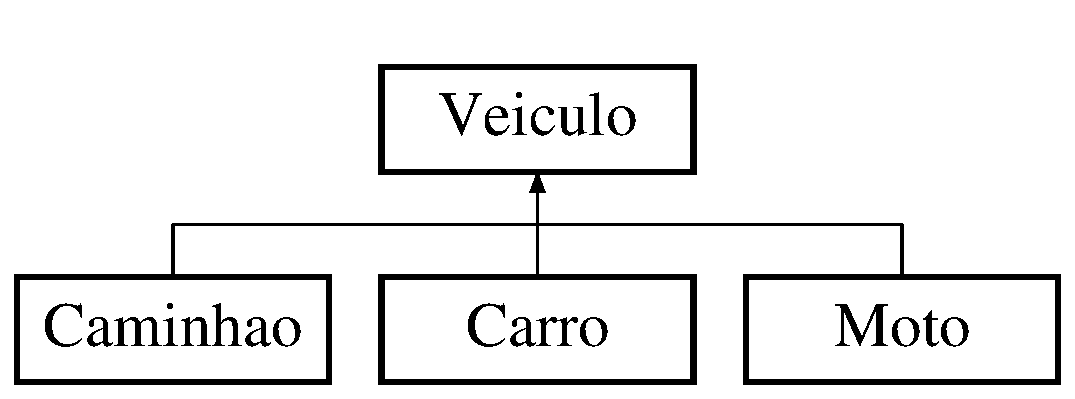
\includegraphics[height=2.000000cm]{class_veiculo}
\end{center}
\end{figure}
\subsection*{Membros Públicos}
\begin{DoxyCompactItemize}
\item 
\mbox{\Hypertarget{class_veiculo_a9e42cc073f5ec6269187d23fbf9f811d}\label{class_veiculo_a9e42cc073f5ec6269187d23fbf9f811d}} 
\mbox{\hyperlink{class_veiculo_a9e42cc073f5ec6269187d23fbf9f811d}{Veiculo}} ()
\begin{DoxyCompactList}\small\item\em Construtor padrão. \end{DoxyCompactList}\item 
\mbox{\hyperlink{class_veiculo_a67a7ce6d304cf4062c642a1071ab0dbf}{Veiculo}} (int \mbox{\hyperlink{class_veiculo_a9a2aef79ea401cf44fd8102e75e4a2de}{speed}}, int \mbox{\hyperlink{class_veiculo_aad500265aeb92689ca66ec5bd87787a9}{cor}})
\item 
\mbox{\Hypertarget{class_veiculo_a84b2207a013e6cd869959b73a93864b8}\label{class_veiculo_a84b2207a013e6cd869959b73a93864b8}} 
void \mbox{\hyperlink{class_veiculo_a84b2207a013e6cd869959b73a93864b8}{setX}} (int \mbox{\hyperlink{class_veiculo_a069917a284297fe5b385258b2afd9ad6}{x}})
\begin{DoxyCompactList}\small\item\em Metodo set para x. \end{DoxyCompactList}\item 
\mbox{\Hypertarget{class_veiculo_a57cb54424b47643d8b388c72dbaf43b1}\label{class_veiculo_a57cb54424b47643d8b388c72dbaf43b1}} 
void \mbox{\hyperlink{class_veiculo_a57cb54424b47643d8b388c72dbaf43b1}{setY}} (int \mbox{\hyperlink{class_veiculo_af25046404db7c2786c0d9e468bb1fb64}{y}})
\begin{DoxyCompactList}\small\item\em Metodo set para y. \end{DoxyCompactList}\item 
\mbox{\Hypertarget{class_veiculo_ae9a07a54a5824a9e8cace2c742034956}\label{class_veiculo_ae9a07a54a5824a9e8cace2c742034956}} 
void \mbox{\hyperlink{class_veiculo_ae9a07a54a5824a9e8cace2c742034956}{set\+Fabrica}} (boolean \mbox{\hyperlink{class_veiculo_a23d377a69bdf558ebedb5bc35dcdebf5}{fabrica}})
\begin{DoxyCompactList}\small\item\em Metodo set para fabrica, true ou false. \end{DoxyCompactList}\item 
\mbox{\Hypertarget{class_veiculo_ae2662b41831f011fc82060ee730b8acb}\label{class_veiculo_ae2662b41831f011fc82060ee730b8acb}} 
void \mbox{\hyperlink{class_veiculo_ae2662b41831f011fc82060ee730b8acb}{set\+Speed}} (int \mbox{\hyperlink{class_veiculo_a9a2aef79ea401cf44fd8102e75e4a2de}{speed}})
\begin{DoxyCompactList}\small\item\em Metodo set para velocidade. \end{DoxyCompactList}\item 
\mbox{\Hypertarget{class_veiculo_ab7fc7e6551ab238df0fb51a1a5c7d66f}\label{class_veiculo_ab7fc7e6551ab238df0fb51a1a5c7d66f}} 
void \mbox{\hyperlink{class_veiculo_ab7fc7e6551ab238df0fb51a1a5c7d66f}{set\+Cor}} (int \mbox{\hyperlink{class_veiculo_aad500265aeb92689ca66ec5bd87787a9}{cor}})
\begin{DoxyCompactList}\small\item\em Metodo set para cor. \end{DoxyCompactList}\item 
\mbox{\Hypertarget{class_veiculo_a235b29e1e25ec8c769b20fb2aeba8404}\label{class_veiculo_a235b29e1e25ec8c769b20fb2aeba8404}} 
int \mbox{\hyperlink{class_veiculo_a235b29e1e25ec8c769b20fb2aeba8404}{getX}} ()
\begin{DoxyCompactList}\small\item\em Metodo get para x. \end{DoxyCompactList}\item 
\mbox{\Hypertarget{class_veiculo_a06b2a923e51186673a016f75d10363d3}\label{class_veiculo_a06b2a923e51186673a016f75d10363d3}} 
int \mbox{\hyperlink{class_veiculo_a06b2a923e51186673a016f75d10363d3}{getY}} ()
\begin{DoxyCompactList}\small\item\em Metodo get para y. \end{DoxyCompactList}\item 
\mbox{\Hypertarget{class_veiculo_a6447f0eeb99399f1f96e835c22a88479}\label{class_veiculo_a6447f0eeb99399f1f96e835c22a88479}} 
boolean \mbox{\hyperlink{class_veiculo_a6447f0eeb99399f1f96e835c22a88479}{get\+Fabrica}} ()
\begin{DoxyCompactList}\small\item\em Metodo get para fabrica, true ou false. \end{DoxyCompactList}\item 
\mbox{\Hypertarget{class_veiculo_a8895a299d223a6d5d9b83c97c8ac1b24}\label{class_veiculo_a8895a299d223a6d5d9b83c97c8ac1b24}} 
int \mbox{\hyperlink{class_veiculo_a8895a299d223a6d5d9b83c97c8ac1b24}{get\+Speed}} ()
\begin{DoxyCompactList}\small\item\em Metodo get para velocidade. \end{DoxyCompactList}\item 
\mbox{\Hypertarget{class_veiculo_a4fed5f48e6ddcf1c3e9a5a5ff9ba3067}\label{class_veiculo_a4fed5f48e6ddcf1c3e9a5a5ff9ba3067}} 
int \mbox{\hyperlink{class_veiculo_a4fed5f48e6ddcf1c3e9a5a5ff9ba3067}{get\+Cor}} ()
\begin{DoxyCompactList}\small\item\em Metodo get para cor. \end{DoxyCompactList}\item 
void \mbox{\hyperlink{class_veiculo_a3341b0ed6b4d34db990a31f7a499ae80}{move}} ()
\end{DoxyCompactItemize}
\subsection*{Atributos Públicos}
\begin{DoxyCompactItemize}
\item 
\mbox{\Hypertarget{class_veiculo_a98ea80a955045a5f578f25fff5b4999a}\label{class_veiculo_a98ea80a955045a5f578f25fff5b4999a}} 
Random \mbox{\hyperlink{class_veiculo_a98ea80a955045a5f578f25fff5b4999a}{gen}} = new Random()
\begin{DoxyCompactList}\small\item\em Gerador de numeros randomicos da biblioteca random. \end{DoxyCompactList}\end{DoxyCompactItemize}
\subsection*{Atributos Protegidos}
\begin{DoxyCompactItemize}
\item 
\mbox{\Hypertarget{class_veiculo_a069917a284297fe5b385258b2afd9ad6}\label{class_veiculo_a069917a284297fe5b385258b2afd9ad6}} 
int \mbox{\hyperlink{class_veiculo_a069917a284297fe5b385258b2afd9ad6}{x}}
\begin{DoxyCompactList}\small\item\em Variavel com valor aleatorio de 0 a 39. \end{DoxyCompactList}\item 
\mbox{\Hypertarget{class_veiculo_af25046404db7c2786c0d9e468bb1fb64}\label{class_veiculo_af25046404db7c2786c0d9e468bb1fb64}} 
int \mbox{\hyperlink{class_veiculo_af25046404db7c2786c0d9e468bb1fb64}{y}}
\begin{DoxyCompactList}\small\item\em Variavel com valor aleatorio de 0 a 39. \end{DoxyCompactList}\item 
\mbox{\Hypertarget{class_veiculo_a23d377a69bdf558ebedb5bc35dcdebf5}\label{class_veiculo_a23d377a69bdf558ebedb5bc35dcdebf5}} 
boolean \mbox{\hyperlink{class_veiculo_a23d377a69bdf558ebedb5bc35dcdebf5}{fabrica}}
\begin{DoxyCompactList}\small\item\em True ou false para saber se cria ou não um veiculo novo. \end{DoxyCompactList}\item 
\mbox{\Hypertarget{class_veiculo_a9a2aef79ea401cf44fd8102e75e4a2de}\label{class_veiculo_a9a2aef79ea401cf44fd8102e75e4a2de}} 
int \mbox{\hyperlink{class_veiculo_a9a2aef79ea401cf44fd8102e75e4a2de}{speed}}
\begin{DoxyCompactList}\small\item\em Velocidade fixa do veiculo. \end{DoxyCompactList}\item 
\mbox{\Hypertarget{class_veiculo_aad500265aeb92689ca66ec5bd87787a9}\label{class_veiculo_aad500265aeb92689ca66ec5bd87787a9}} 
int \mbox{\hyperlink{class_veiculo_aad500265aeb92689ca66ec5bd87787a9}{cor}}
\begin{DoxyCompactList}\small\item\em Cor fixa de um veiculo. \end{DoxyCompactList}\end{DoxyCompactItemize}


\subsection{Descrição detalhada}
Classe \mbox{\hyperlink{class_veiculo}{Veiculo}}. Tem como função criar um objeto \mbox{\hyperlink{class_veiculo}{Veiculo}} que é chamado pelas classes herdadas. 

\subsection{Construtores e Destrutores}
\mbox{\Hypertarget{class_veiculo_a67a7ce6d304cf4062c642a1071ab0dbf}\label{class_veiculo_a67a7ce6d304cf4062c642a1071ab0dbf}} 
\index{Veiculo@{Veiculo}!Veiculo@{Veiculo}}
\index{Veiculo@{Veiculo}!Veiculo@{Veiculo}}
\subsubsection{\texorpdfstring{Veiculo()}{Veiculo()}}
{\footnotesize\ttfamily Veiculo.\+Veiculo (\begin{DoxyParamCaption}\item[{int}]{speed,  }\item[{int}]{cor }\end{DoxyParamCaption})\hspace{0.3cm}{\ttfamily [inline]}}

Um construtor parametrizado. Cria um veiculo que recebe das suas subclasses a velocidade e a cor que o representa. chama o metodo set entrando um numero aleatorio de 0 a 39.

chama o metodo set entrando um numero aleatorio de 0 a 39.

chama o metodo set entrando o boolean false como padrão.

chama o metodo set entrando a velocidade oferecida por uma das subclasses do \mbox{\hyperlink{class_veiculo}{Veiculo}}.

chama o metodo set entrando a cor oferecida por uma das subclasses do \mbox{\hyperlink{class_veiculo}{Veiculo}}. 

\subsection{Funções membros}
\mbox{\Hypertarget{class_veiculo_a3341b0ed6b4d34db990a31f7a499ae80}\label{class_veiculo_a3341b0ed6b4d34db990a31f7a499ae80}} 
\index{Veiculo@{Veiculo}!move@{move}}
\index{move@{move}!Veiculo@{Veiculo}}
\subsubsection{\texorpdfstring{move()}{move()}}
{\footnotesize\ttfamily void Veiculo.\+move (\begin{DoxyParamCaption}{ }\end{DoxyParamCaption})\hspace{0.3cm}{\ttfamily [inline]}}

Metodo para mover o \mbox{\hyperlink{class_veiculo}{Veiculo}} de forma aleatoria, utilizando a biblioteca random. $<$ variavel com valor aleatorio entre 1 e 4.

Confirma se x e y estão de acordo com o tamanho do mundo. 

A documentação para essa classe foi gerada a partir do seguinte arquivo\+:\begin{DoxyCompactItemize}
\item 
C\+:/\+Users/\+User/\+Documents/\+Git\+Hub/\+Projeto\+P1\+\_\+\+J\+A\+V\+A/src/Veiculo.\+java\end{DoxyCompactItemize}

%--- End generated contents ---

% Index
\backmatter
\newpage
\phantomsection
\clearemptydoublepage
\addcontentsline{toc}{chapter}{Sumário}
\printindex

\end{document}
